% presentation.tex
% gscore — a talk
%
% (C) Copyright 2026 Sebastien Tricaud
%
% Build:
%     cd docs && pdflatex presentation.tex && pdflatex presentation.tex
%
% Twice, for the slide numbers. Every picture comes out of the repository —
% the icon, Gilbert, and a screenshot of the 2005 program rescued from the
% Internet Archive — so there is nothing to fetch and nothing to install.

\documentclass[aspectratio=169,12pt]{beamer}

\usepackage[T1]{fontenc}
\usepackage[utf8]{inputenc}
\usepackage{lmodern}
\usepackage{graphicx}
\usepackage{tikz}
\usepackage{wasysym}  % \quarternote, for quoting a tempo marking

\graphicspath{{../assets/icon/}{../internal/brand/}{../assets/history/}{../assets/}}

%% ---------------------------------------------------------------- theme

\usetheme{default}
\usecolortheme{default}
\setbeamertemplate{navigation symbols}{}

\definecolor{ink}{HTML}{1A1A1A}
\definecolor{paper}{HTML}{FBFAF7}
\definecolor{accent}{HTML}{1F6FB2}
\definecolor{quiet}{HTML}{6B6B6B}
\definecolor{old}{HTML}{8A6D3B}

\setbeamercolor{normal text}{fg=ink,bg=paper}
\setbeamercolor{structure}{fg=accent}
\setbeamercolor{frametitle}{fg=ink}
\setbeamerfont{frametitle}{size=\LARGE,series=\bfseries}

% A title that sits on the page rather than in a coloured bar, and the
% mascot in the corner of every slide. He has earned it.
\setbeamertemplate{frametitle}{%
  \vspace{0.7em}\insertframetitle\par
  {\color{accent}\rule{\textwidth}{1.2pt}}\par\vspace{-0.4em}}

\setbeamertemplate{footline}{%
  \hfill
  \raisebox{0.6em}{\color{quiet}\footnotesize\insertframenumber}%
  \hspace{1em}%
  \raisebox{0.2em}{
\includegraphics[height=1.6em]{gilbert}}%
  \hspace{1.2em}\vspace{0.4em}}

%% Gilbert is the bullet. He was the splash screen in 2005 and he is the
%% thing people remember, so he does the pointing.
\newcommand{\gilbertbullet}{\raisebox{-0.22ex}{
\includegraphics[height=1.5ex]{gilbert}}}
\setbeamertemplate{itemize item}{\gilbertbullet}
\setbeamertemplate{itemize subitem}{\raisebox{-0.15ex}{
\includegraphics[height=1.1ex]{gilbert}}}
\setbeamertemplate{itemize subsubitem}{\raisebox{-0.12ex}{
\includegraphics[height=0.9ex]{gilbert}}}
\setlength{\leftmargini}{2.2em}
\setlength{\leftmarginii}{2em}

\newcommand{\key}[1]{%
  \tikz[baseline=(k.base)]{
    \node[draw=quiet,rounded corners=2pt,inner xsep=4pt,inner ysep=2pt,
          fill=white,font=\small\ttfamily] (k) {#1};}}

\newcommand{\hi}[1]{{\color{accent}\textbf{#1}}}
\newcommand{\punch}[1]{\begin{center}{\large #1}\end{center}}

\title{gscore}
\author{Sébastien Tricaud}
\date{}

\begin{document}

%% ---------------------------------------------------------------- title

{\setbeamertemplate{footline}{}
\begin{frame}[plain]
  \vfill
  \begin{center}
    
\includegraphics[height=0.3\textheight]{gscore}\\[1.1em]
    {\Huge\bfseries gscore}\\[0.6em]
    {\large\color{quiet} Sheet music anyone can open}\\[2.0em]
    {\color{quiet}\small Sébastien Tricaud \quad·\quad GPL v2 or later \quad·\quad since 2001}
  \end{center}
  \vfill
\end{frame}}

%% ---------------------------------------------------------------- 2001

\begin{frame}{June 2001}
  \vspace{0.5em}
  A man. A Linux box. GTK+. No plan to speak of.
  \vspace{1.0em}

  The very first line of the changelog:
  \vspace{0.6em}
  \begin{center}
  \begin{minipage}{0.86\textwidth}
    \color{old}\ttfamily\small
    2001-06-03\quad toady\\[0.3em]
    \hspace*{1.2em}* src/main.c: You can exit the app using X-kill with a\\
    \hspace*{3.4em} dialog asking you for the modifications you did (arf!).
  \end{minipage}
  \end{center}
  \vspace{0.9em}
  \punch{Four years and \hi{15{,}627 lines of C} later, it could write music.}
\end{frame}

%% ---------------------------------------------------------------- 0.0.9

\begin{frame}{This is gscore 0.0.9, April 2005}
  \vspace{0.2em}
  \begin{center}
    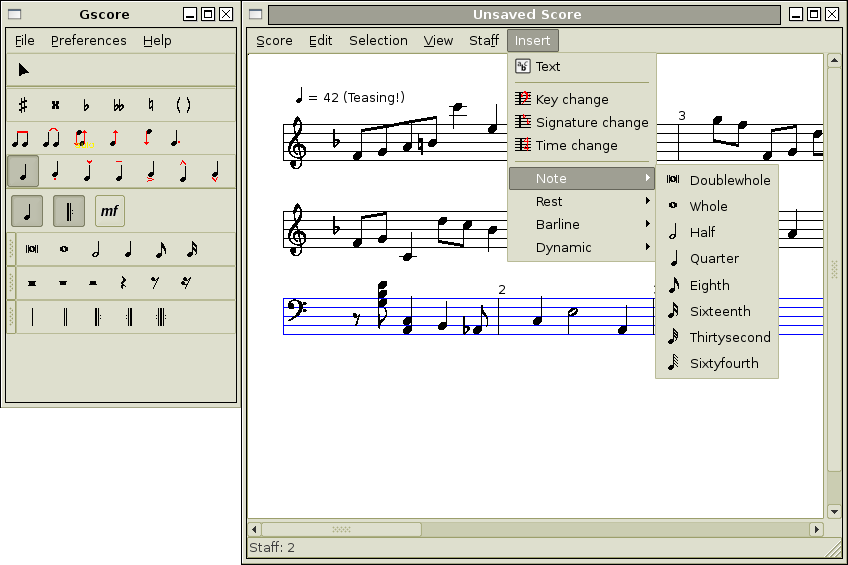
\includegraphics[height=0.64\textheight]{gscore-0.0.9}
  \end{center}
  \vspace{-0.3em}
  \begin{center}\color{quiet}\small
    A floating toolbox, because GIMP did it that way and GIMP was right.
  \end{center}
\end{frame}

\begin{frame}{Look closely at that screenshot}
  \vspace{0.4em}
  \begin{itemize}\setlength\itemsep{0.85em}
    \item The music runs on and on --- \hi{no pages, no page breaks}
    \item Because it was for \emph{writing}, not for printing
    \item The tempo marking in the demo score reads \hi{``\quarternote{} = 42 (Teasing!)''}
    \item Somebody was enjoying themselves
  \end{itemize}
  \vspace{0.9em}
  \punch{Twenty-one years later, that strip is still in there.\\
  It is called \hi{Continuous} and it is still the better way to write.}
\end{frame}

\begin{frame}{Releases had names, naturally}
  \vspace{1.2em}
  \begin{center}
    {\large 0.0.7 \quad\textemdash\quad \hi{``bond''}}\\[1.1em]
    {\large 0.0.9 \quad\textemdash\quad \hi{``harder, better, stronger, faster''}}
  \end{center}
  \vspace{1.4em}
  \begin{center}
  \begin{minipage}{0.92\textwidth}
    \color{old}\ttfamily\footnotesize
    * src/score.c: Replace ``set header'' glade widget with a custom one\\
    \hspace*{1.2em} to make the release in 2005 and\\
    \hspace*{1.2em} \textbf{stop fighting with glade for MDI stuff}
  \end{minipage}
  \end{center}
  \vspace{1.2em}
  \punch{\color{quiet}Every programmer has written that commit.}
\end{frame}

%% ---------------------------------------------------------------- pause

\begin{frame}{Then: twenty-one years of silence}
  \vspace{0.7em}
  \begin{itemize}\setlength\itemsep{0.9em}
    \item Mandrake packaged it in December 2004
    \item Mandriva kept packaging it
    \item \hi{OpenMandriva still ships it today}
    \item Nobody told the maintainers to stop, so they did not
  \end{itemize}
  \vspace{1.0em}
  \punch{A program can outlive its own author's attention span.}
\end{frame}

%% ---------------------------------------------------------------- 2026

\begin{frame}{2026: written again, from nothing}
  \vspace{0.3em}
  \begin{columns}[T]
    \begin{column}{0.62\textwidth}
      \begin{itemize}\setlength\itemsep{0.6em}
        \item Go instead of C
        \item SMuFL and Bravura instead of hand-drawn pixmaps
        \item Tests instead of hope
        \item The 2005 source kept intact as the specification
        \item \hi{Gilbert survived the rewrite}
      \end{itemize}
    \end{column}
    \begin{column}{0.33\textwidth}
      \begin{center}
        
\includegraphics[height=0.34\textheight]{gilbert}\\[0.6em]
        {\color{quiet}\small He was the splash screen.\\He is now the bullet point.}
      \end{center}
    \end{column}
  \end{columns}
  \vspace{0.4em}
  \punch{Same idea. Same mascot. Rather better engraving.}
\end{frame}

%% ---------------------------------------------------------------- problem

\begin{frame}{So. You have written a piece.}
  \vspace{0.8em}
  Now send it to your flute player.
  \vspace{1.0em}
  \begin{itemize}\setlength\itemsep{0.8em}
    \item ``Install MuseScore first.'' \hfill \textit{\color{quiet}half a gigabyte and an account}
    \item ``Here's a PDF.'' \hfill \textit{\color{quiet}now it is a picture}
    \item ``It's on this website.'' \hfill \textit{\color{quiet}adverts, login, link rot}
    \item ``What on earth is a \texttt{.mscz}?'' \hfill \textit{\color{quiet}a fair question}
  \end{itemize}
  \vspace{1.2em}
  \punch{Writing the music was the \emph{easy} part.}
\end{frame}

%% ---------------------------------------------------------------- answer

\begin{frame}{One file. Everyone can open it.}
  \vspace{0.5em}
  \begin{center}
    {\Large\ttfamily badinerie.html}
  \end{center}
  \vspace{1.3em}
  \begin{itemize}\setlength\itemsep{0.75em}
    \item Double-click. It opens in \hi{any browser ever made}
    \item The engraving, the music font and the player are \hi{inside the file}
    \item No install. No server. No account. No network.
    \item Your phone. The work laptop nobody may install things on. 2036.
  \end{itemize}
\end{frame}

\begin{frame}{\dots and then it plays}
  \vspace{1.0em}
  \begin{itemize}\setlength\itemsep{0.9em}
    \item Press play \emph{in the page}: it sounds, and the cursor follows along
    \item Slurs held, staccato short, dynamics where you put them
    \item Nothing downloads --- the sound is in there too
  \end{itemize}
  \vspace{1.6em}
  \punch{You did not send a picture of a score.\\
  You sent \hi{the score}.}
\end{frame}

%% ---------------------------------------------------------------- pdf

\begin{frame}{The file that is also a different file}
  \vspace{0.6em}
  \begin{center}
    {\large\ttfamily sonata.gscore}\\[0.5em]
    {\large $\downarrow$ \ \color{quiet}rename it}\\[0.5em]
    {\large\ttfamily sonata.pdf}
  \end{center}
  \vspace{1.2em}
  \begin{itemize}\setlength\itemsep{0.7em}
    \item A saved score carries a printed PDF of itself in front of it
    \item Renamed, it opens in anything that reads a PDF
    \item Opened in gscore, it is still the \hi{editable score}
  \end{itemize}
  \vspace{0.7em}
  \punch{\color{quiet}One file to keep. One file to send. They are the same file.}
\end{frame}

%% ---------------------------------------------------------------- parts

\begin{frame}{Parts your players will not complain about}
  \vspace{0.7em}
  \begin{itemize}\setlength\itemsep{0.75em}
    \item One PDF: the conductor's score, then every instrument behind it
    \item Score on its side if that is what holds it --- \hi{parts always upright}
    \item Each part set at a size readable from a stand, not from a microscope
    \item Each part named in its own margin, pages numbered \emph{within itself}
    \item Seventeen staves too tall for the sheet? Divided \hi{between staves}, evenly --- never sliced off by the paper's edge
  \end{itemize}
\end{frame}

%% ---------------------------------------------------------------- speed

\begin{frame}{Writing music is typing}
  \vspace{0.2em}
  \begin{columns}[T]
    \begin{column}{0.5\textwidth}
      \begin{itemize}\setlength\itemsep{0.6em}
        \item \key{$\uparrow$} \key{$\downarrow$} \ move the note a step
        \item \key{space} \ write it
        \item \key{enter} \ a rest, same length
        \item \key{$\leftarrow$} \key{$\rightarrow$} \ move along
        \item \key{backspace} \ undo your optimism
      \end{itemize}
    \end{column}
    \begin{column}{0.46\textwidth}
      \begin{itemize}\setlength\itemsep{0.6em}
        \item \key{b} beam \ \ \key{S} slur \ \ \key{=} tie
        \item \key{u} \key{d} stem up, stem down
        \item \key{.} dot it
        \item \key{shift}+\key{space} play
        \item \key{esc} back to the top
      \end{itemize}
    \end{column}
  \end{columns}
  \vspace{1.0em}
  \punch{\color{quiet}Your hands never leave the keyboard. Neither does your attention.}
\end{frame}

\begin{frame}{The number row \emph{is} the note value}
  \vspace{1.3em}
  \begin{center}
    \begin{tabular}{llll}
      \key{1} whole & \key{2} half & \key{3} dotted half & \key{4} quarter \\[0.9em]
      \key{5} dotted quarter & \key{8} eighth & \key{9} sixteenth & \key{0} thirty-second \\
    \end{tabular}
  \end{center}
  \vspace{1.5em}
  \begin{itemize}\setlength\itemsep{0.7em}
    \item Pick a length, type the tune, change the length, carry on
    \item On a drum staff the \hi{letters type the kit} --- a groove is typed, not clicked thirty-two times
  \end{itemize}
\end{frame}

%% ---------------------------------------------------------------- platform

\begin{frame}{Everywhere. And it is one file.}
  \vspace{0.4em}
  \begin{itemize}\setlength\itemsep{0.8em}
    \item \hi{macOS} --- a real Mac application, menu bar and all
    \item \hi{Windows} --- one \texttt{.exe}; put it anywhere, run it
    \item \hi{Linux} --- a \texttt{.deb}, or the same single binary
    \item \hi{A web page} --- the entire program compiled to WebAssembly.
      No server. Your music never leaves your machine.
  \end{itemize}
  \vspace{1.1em}
  \punch{\color{quiet}The interface, the music font and the engraver all live inside the binary.\\
  There is nothing to install beside it. There never was.}
\end{frame}

%% ---------------------------------------------------------------- reads

\begin{frame}{It opens what you already have}
  \vspace{0.8em}
  \begin{itemize}\setlength\itemsep{0.7em}
    \item \texttt{.mscz} \ \texttt{.mscx} \hfill \textit{\color{quiet}MuseScore, without MuseScore}
    \item \texttt{.musicxml} \ \texttt{.xml} \ \texttt{.mxl} \hfill \textit{\color{quiet}from anything at all}
    \item \texttt{.nwc} \ \texttt{.nwctxt} \hfill \textit{\color{quiet}NoteWorthy, without Windows}
    \item \texttt{.abc} \hfill \textit{\color{quiet}the entire folk archive}
  \end{itemize}
  \vspace{1.3em}
  \punch{Every importer reads \emph{past} what it does not understand\\
  and then tells you what it skipped.\\[0.4em]
  \hi{A file is never refused whole.}}
\end{frame}

\begin{frame}{And writes what everybody else reads}
  \vspace{0.9em}
  \begin{columns}[T]
    \begin{column}{0.47\textwidth}
      \begin{itemize}\setlength\itemsep{0.65em}
        \item \hi{PDF} --- print it
        \item \hi{HTML} --- send it
        \item \hi{MusicXML} --- anywhere
        \item \hi{SVG} --- into a document
      \end{itemize}
    \end{column}
    \begin{column}{0.47\textwidth}
      \begin{itemize}\setlength\itemsep{0.65em}
        \item \hi{MIDI} --- into your DAW
        \item \hi{FLAC} --- a real recording
        \item \hi{LilyPond} --- for engraving even better than this
      \end{itemize}
    \end{column}
  \end{columns}
  \vspace{1.3em}
  \punch{\color{quiet}The LilyPond export is tested by \emph{compiling it with LilyPond}.\\
  Saying ``it looks like LilyPond'' is not a claim worth making.}
\end{frame}

%% ---------------------------------------------------------------- sound

\begin{frame}{It sounds like actual instruments}
  \vspace{0.9em}
  \begin{itemize}\setlength\itemsep{0.8em}
    \item Press play: you hear it \emph{immediately} --- no loading, no waiting
    \item Point it at a soundfont and it plays \hi{real recorded instruments}
    \item The Mac and Windows downloads \hi{already carry one}
    \item Export the whole score as FLAC, losslessly
  \end{itemize}
  \vspace{1.2em}
  \punch{\color{quiet}One place in the program decides what the music sounds like,\\
  so the editor, the MIDI file and the recording cannot disagree.}
\end{frame}

%% ---------------------------------------------------------------- symbols

\begin{frame}{Invent a mark. Send it to someone.}
  \vspace{0.9em}
  \begin{itemize}\setlength\itemsep{0.85em}
    \item Draw it, name it, put it on a note
    \item It \hi{travels inside the file}, still attached to that note
    \item They open the score; the mark is there, and it still means something
    \item Share a whole set of them as a pack
  \end{itemize}
  \vspace{1.4em}
  \punch{Everywhere else, an invented mark arrives as\\
  a \emph{smudge floating near the music}.}
\end{frame}

%% ---------------------------------------------------------------- close

{\setbeamertemplate{footline}{}
\begin{frame}[plain]
  \vfill
  \begin{center}
    
\includegraphics[height=0.26\textheight]{gilbert}\\[1.1em]
    {\LARGE\bfseries One file. Anyone can open it.}\\[1.5em]
    {\large\ttfamily github.com/stricaud/gscore}\\[1.2em]
    {\color{quiet}\small
      C and GTK+, 2001--2005. Go, 2026.\\
      Gilbert, throughout.}
  \end{center}
  \vfill
\end{frame}}

\end{document}
